\documentclass[12pt]{article}
\usepackage[utf8]{inputenc}
\usepackage{amsmath}
\usepackage{mathtools}
\usepackage{amsfonts}
\usepackage{lastpage}
\usepackage{tikz}
\usepackage{pdfpages}
\usepackage{gauss}
\usepackage{fancyvrb}
\usepackage{fancyhdr}
\usepackage{graphicx}
\pagestyle{fancy}
\fancyfoot[C]{\footnotesize Page \thepage\ of 8}
\DeclareGraphicsExtensions{.pdf,.png,.jpg}
\title{MatIntroNat}
\author{Nikolaj Dybdahl Rathcke}
\chead{Nikolaj Dybdahl Rathcke (rfq695)}

\begin{document}
\section*{MatIntroNat - Opgave 3}

\subsection*{Opgave 5.1}
Betragt funktionen $f(x,y)=\sqrt{4xy-3y^2}$.\\

\subsubsection*{a}
Bestem definitionsmængden $D_f$. Skitser, uden Maple, $D_f$ i et \textit{xy}-diagram.\\
\\
Definitionsmængden er givet ved kombinationerne der ikke giver et negativt tal under kvadratroden, altså
$$4xy-3y^2\geq 0$$
Dette kan vi faktorisere til
$$y(4x-3y)\geq 0$$
Kigger vi på løsninger for $y\geq 0$ ses at parentesen bliver ganget med et positivt tal og derfor skal der blot gælde
$$4x-3y\geq 0$$
$$4x\geq 3y$$
$$x\geq \frac{3}{4}y$$
For løsninger for $y<0$ bliver der multipliceret med et negativt tal, altså skal parentesen også være negativ eller 0 for at hele venstre side er positiv eller 0, så der skal gælde
$$4x-3y\leq 0$$
$$4x\leq 3y$$
$$x\leq \frac{3}{4}y$$
Altså er definitionsmængden, $D_f$, bestemt ved
$$D_f=(x\geq \frac{3}{4}y\:\wedge\:y\geq 0)\:\vee\:(x\leq \frac{3}{4}y\:\wedge\:y<0)$$
Definitionsmængden er skitseret på bilag 1, hvor det er de markerede områder.

\subsubsection*{b}
Lav, med Maple, et \textbf{plot3d} af funktionen $4xy-3y^2$, og sammensæt dette med et plot af \textit{xy}-planen, således at uligheden $4xy-3y^2\geq 0$ illustreres.\\
\\
Nedenfor ses et plot3d i Maple\\
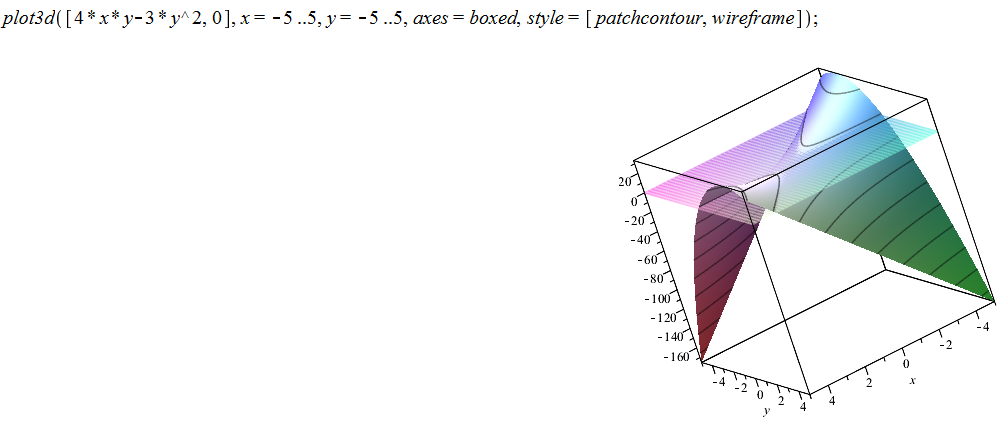
\includegraphics[scale=0.6]{Pic2}\\
hvor uligheden $4xy-3y^2\geq 0$ er illustreret.

\subsubsection*{c}
Bestem, uden Maple, $lim_{h\rightarrow 0^{+}}\frac{f(h,rh)}{h}$ for alle $r\in [0,\frac{4}{3}]$.\\
\\
Vi kan opskrive brøken $\frac{f(h,rh)}{h}$ som
$$\frac{\sqrt{4hrh-3(rh)^2}}{h}$$
Hvor vi kan omskrive hele brøken
$$\frac{\sqrt{4h^2r-3h^2r^2}}{h}$$
$$\frac{h\sqrt{4r-3r^2}}{h}$$
Og da vi nu helt kan fjerne $h$ fra brøken kan vi opskrive grænseværdien som 
$$lim_{h\rightarrow0^{+}}\frac{f(h,rh)}{h}=\sqrt{4r-3r^2}$$
Vi ønsker desuden at vise at der er en grænseværdi for alle $r\in [0,\frac{4}{3}]$ hvilket den er så længe udtrykket i kvadratroden ikke er negativ.\\
Vi finder derfor løsningerne til $-3r^2+4r=0$
$$\frac{-b\pm \sqrt{b^2-4ac}}{2a}$$
$$\frac{-4\pm \sqrt{4^2-4*(-3)*0}}{2*(-3)}$$
$$\frac{-4\pm 4}{-6}$$
Hvoraf vi ser løsningerne
$$r1=\frac{-4+4}{-6}=0$$
$$r2=\frac{-4-4}{-6}=\frac{4}{3}$$
Desuden ved indsættelse af $r=1$ i ligningen er
$$4r-3r^2=4*1-3*1^2=1$$
Altså må alle værdier i intervallet $[0,\frac{4}{3}]$ være ikke-negative og derved er der en grænseværdi for alle $r\in [0,\frac{4}{3}]$, nemlig
$$lim_{h\rightarrow0^{+}}\frac{f(h,rh)}{h}=\sqrt{4r-3r^2}$$
som fundet tidligere.

\newpage

\subsection*{Opgave 5.2}

\subsubsection*{a}
Bestem alle Taylorpolynomierne omkring $x=1$ for funktionen $f(x)=x^4 +7x^2-2$ for (uden Maple)\\
\\
Vi ser at det er et 4. grads polynomie, og altså kan det differentieres 5 gange
$$f\prime(x)=4x^3+14x$$
$$f\prime\prime(x)=12x^2+14$$
$$f\prime\prime\prime(x)=24x$$
$$f\prime\prime\prime\prime(x)=24$$
$$f\prime\prime\prime\prime\prime(x)=0$$
Derefter bruger vi definition 11.1.2 i TL, til at opskrive Taylorpolynomierne omkring $x=1$
$$T_nf(x)=\frac{6}{0!}+\frac{18x-18}{1!}+\frac{26x^2-52x+26}{2!}+\frac{24x^3-72x^2+72x-24}{3!}$$
$$+\frac{24x^4-96x^3+144x^2-96x+24}{4!}+0$$
Dette skriver vi op som
$$T_0f=6$$
$$T_1f=18x-12$$
$$T_2f=13x^2-8x+1$$
$$T_3f=4x^3+x^2+4x-3$$
$$T_4f=x^4+7x^2-2$$
Som er Taylorpolynomierne omkring $x=1$.

\subsubsection*{b}
Indtegn (med Maple) resultatet resultatet fra (a) i et plot, som viser grafen for $f$ samt de tre Taylorpolynomier $T_1f, T_2f$ og $T_3f$. Vælg f.eks. $x$-intervallet $[3,-3]$.\\
\\
Nedenfor ses plottet for $f$ samt de første 3 Taylorpolynomier.\\
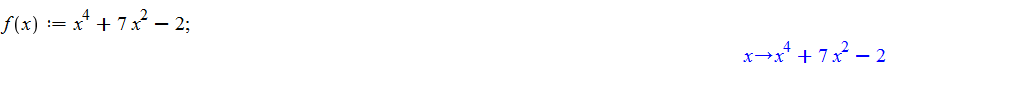
\includegraphics[scale=0.6]{Pic3}\\
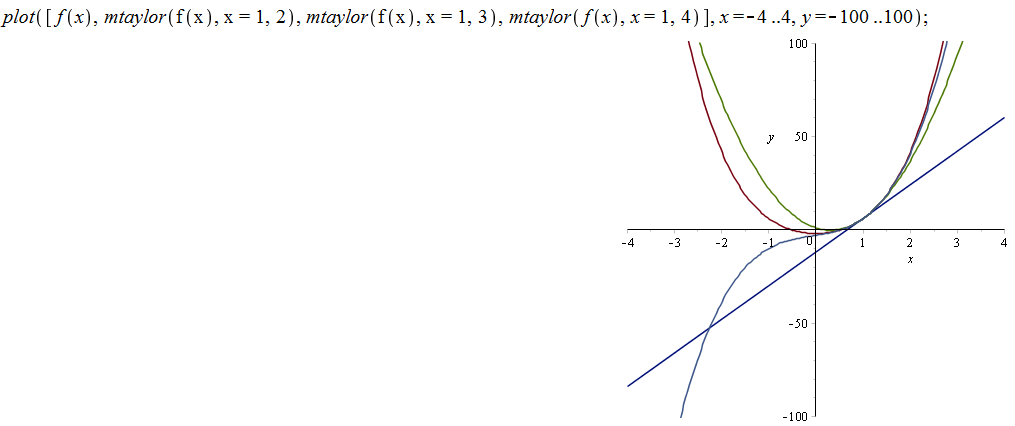
\includegraphics[scale=0.6]{Pic1}\\
Her er mørkeblå grafen for $T_1f$, grøn er grafen for $T_2f$, lyseblå er grafen for $T_3f$ og rød er grafen for $f$.

\newpage

\subsection*{Opgave 5.3(i)}
Betragt den naturlige logaritmefunktion $f(x)=ln(x)$, og lad $T_n$ln være Taylorpolynomiet af grad $n$ omkring $x=1$. Benyt formlen for den $n$-te afledte af $ln$, $f^{(n)}(x)=(-1)^{n-1}(n-1)!x^{-n}$.

\subsubsection*{a}
Plot, med Maple, graferne for ln, $T_9$ln og $T_{49}$ln i et fælles plot.\\
\\
Nedenfor ses det fælles plot\\
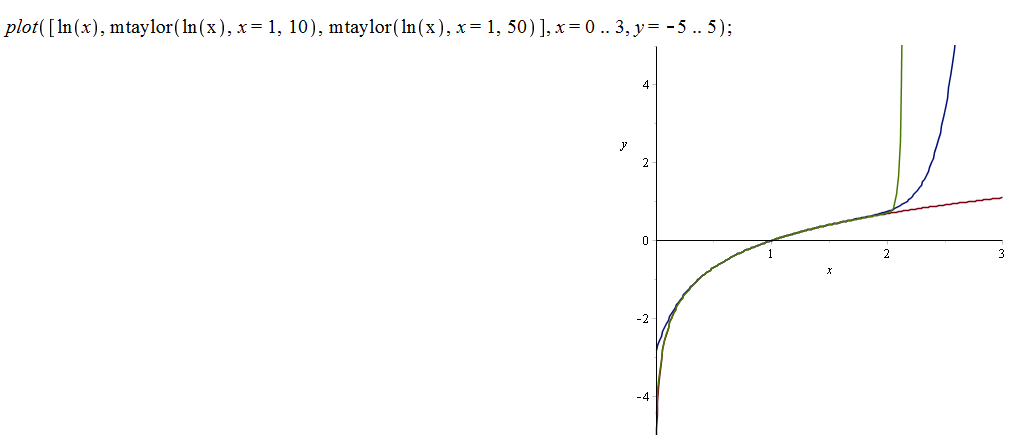
\includegraphics[scale=0.6]{Pic4}\\
hvor den røde er grafen for $ln$, den mørkeblå grafen for $T_9ln$ og den grønne er grafen for $T_{49}ln$.

\subsubsection*{b}
Argumenter, ud fra Taylors formel med restled, for at
$$|R_nln(x)|=|ln(x)-T_nln(x)|\leq\frac{1}{n+1}(x-1)^{n+1}$$
for $x>1$. Udregn, med Maple, for $x=2$, $x=1.9$, $x=2.1$, værdien af $T_{49}ln(x)$ og sammenlign med $ln(x)$. Forklar forskellen mellem tilfældene $x<2$ og $x>2$.\\
\\
Vi benytter os a varianten 'Lagranges restledsformel' som ser ud på følgende måde$$R_nf(x)=\frac{f^{(n+1)}(c)}{(n+1)!}(x-a)^{n+1}$$
Vi har desuden at
$$f^{n+1}ln(x)=(-1)^nn!x^{-(n+1)}$$
Derfor kan vi skrive restleddet med $a=1$ som
$$R_nln(x)=\frac{(-1)^nn!c^{-(n+1)}}{(n+1)!}(x-1)^{n+1}$$
$$R_nln(x)=\frac{(-1)^nc^{-(n+1)}}{n+1}(x-1)^{n+1}$$
$$R_nln(x)=\frac{\frac{(-1)^n}{c^{n+1}}}{n+1}(x-1)^{n+1}$$
\\
Da vi desuden har at $c$ ligger mellem $a$ og $x$ af Lagranges restformel samt $x>1$. Dette betyder at
$$|\frac{(-1)^n}{c^{n+1}}|\leq1$$
Og derfra kan vi udlede at
$$|R_nln(x)|=|\frac{\frac{(-1)^n}{c^{n+1}}}{n+1}(x-1)^{n+1}|\leq\frac{1}{n+1}(x-1)^{n+1}$$
Eller blot
$$|R_nln(x)|=|ln(x)-T_nln(x)|\leq\frac{1}{n+1}(x-1)^{n+1}$$
hvilket er hvad vi ønskede at vise.\\
\\
Vi beregner nu $T_{49}ln(x)$ for $x=2$ samt $ln(2)$\\
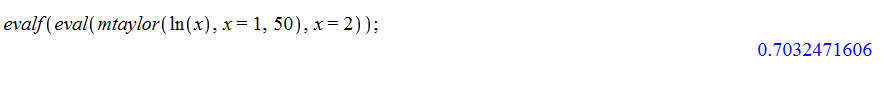
\includegraphics[scale=0.6]{Pic5}\\
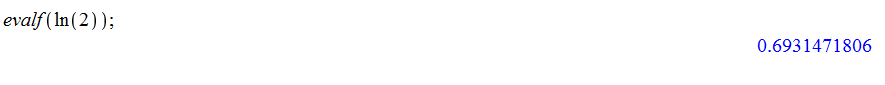
\includegraphics[scale=0.6]{Pic8}\\
Dernæst for $x=1.9$ samt $ln(1.9)$\\
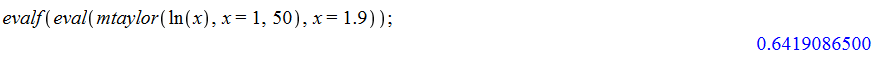
\includegraphics[scale=0.6]{Pic6}\\
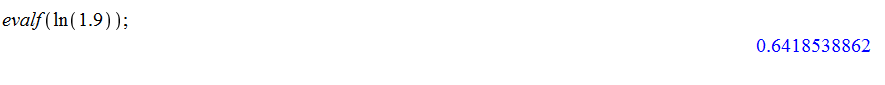
\includegraphics[scale=0.6]{Pic9}\\
Og for $x=2.1$ samt $ln(2.1)$\\
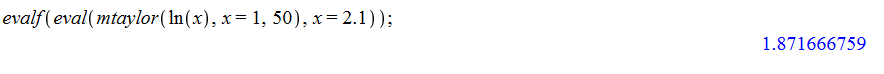
\includegraphics[scale=0.6]{Pic7}\\
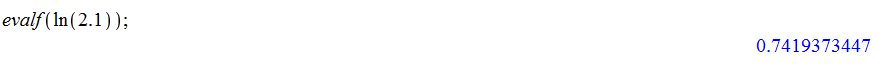
\includegraphics[scale=0.6]{Pic10}\\
Når vi kigger på udtrykket for den øvre begrænsning for restleddet
$$\frac{1}{n+1}(x-1)^{n+1}$$
ses at når $x=2$ vil hele leddet $(x-1)^{n+1}$ altid være lig 1 og dette vil altså ikke have en effekt hele restleddet.\\
Ser vi på $x<2$ ses at $(x-1)^n+1$ vil blive mindre end 1 og derfor vil hele udtrykket for restleddet være mindre.\\
For $x>2$ er $(x-1)^{n+1}$ være større end 1 og hele udtrykket for restleddet vil derfor blive større.\\
Dette er også tilfældet når vi kigger på vores udregnede værdier.

\end{document}
